	\subsection{Pochodzenie danych}
Dane używane przez nas do algorytmu to para liczb - cena mieszkania oraz jego ilość metrów kwadratowych. Wszystkie dane zostały spisane z ogólnodostępnej strony otodom, gdzie każdy może wystawić mieszkanie na sprzedaż. Nie było żadnych innych kryteriów od tego, aby mieszkanie znajdowało się we Wrocławiu - są tu jednocześnie mieszkania używane jak i nowe budownictwo. Link do srony, z której zostały pobrane dane:
\\
\\
\url{https://www.otodom.pl/sprzedaz/mieszkanie/wroclaw/}
\\
\\
Zebranych zostało 53 przykładów danych, z tego 3 zostaną przeznaczone na odrzucenie najbardziej odbiegających danych - jest to celowy zabieg, który pozwala usunąć około 5\% wyników, które znacząco odbiegają od normy oraz mogą spowodować niepoprawne nauczenie algorytmu, co jest równoznaczne ze źle wyznaczoną regresją liniową. Wszystkie dane zostały zebrane losowo, nie były w żaden sposób poddane modyfikacji oraz selekcji wstępnej.
	\subsection{Zoobrazowanie zbioru danych}
Na poniższym wykresie przedstawiono wszystkie dane, które zostały zebrane. Jest to 53 punktów, dla których położenie jest określone poprzez wartość na osi ceny oraz powierzchni mieszkania.

	\begin{figure}[H]
    \centering
    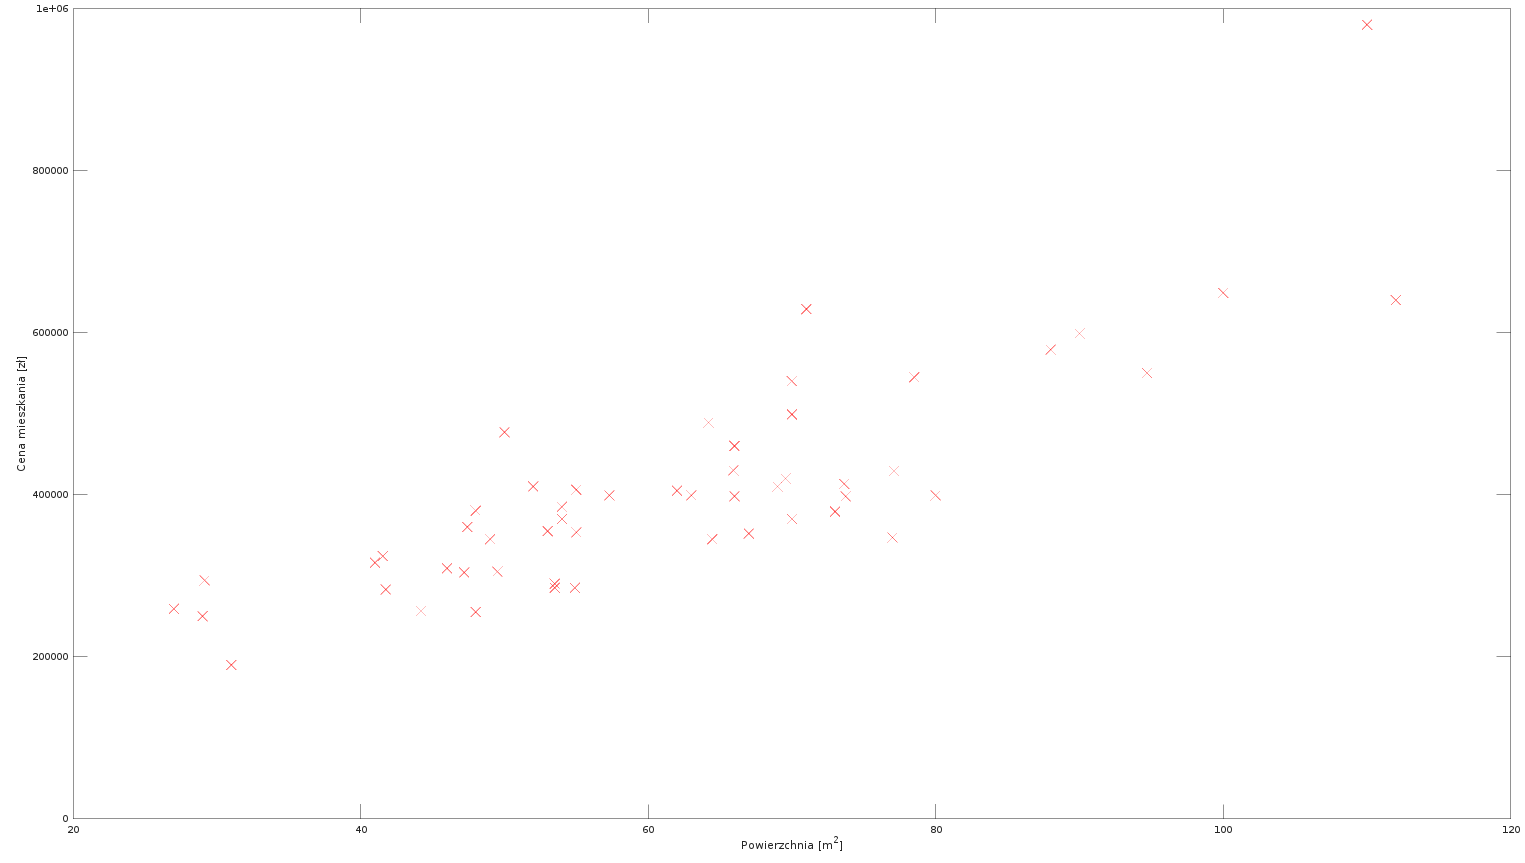
\includegraphics[scale=0.24]{PNG/y_X.png}
    \caption{Surowy zbiór danych}
    \label{lamana}
	\end{figure}
	
Wszystkie dane z powyższego wykresu zostały również zebrane w poniższej tabeli. Są one ułozone w sposób nieposortowane - dokładnie w takiej samej kolejności w jakiej zostały znalezione w wyszukiwarce otodom.pl. Przy cenach mieszkań zostały odcięte wartości po przecinku, natomiast wartości powierzchni zostały niezmienione względem danych podanych na stronie - dane te mogę być lekko różne od prawdziwego stanu w danym mieszkaniu.\\

\begin{tabular}{|c|c|c|c|}
	\hline
	Cena lokalu & Powierzchnia & Cena lokalu & Powierzchnia\\
	\hline
	[zł] & [$m^{2}$] & [zł] & [$m^{2}$]\\
	\hline
649 000 & 100.00 & 399 000 & 63.00\\
	\hline
550 000 & 94.70 & 353 376 & 55.00\\
	\hline
499 000 & 70.00 & 355 000 & 53.00\\
	\hline
540 000 & 70.00 & 599 000 & 90.00\\
	\hline
309 000 & 46.00 & 259 000 & 27.00\\
	\hline
489 000 & 64.20 & 410 000 & 52.00\\
	\hline
460 000 & 66.00 & 399 000 & 80.00\\
	\hline
351 972 & 67.00 & 398 000 & 73.73\\
	\hline
413 200 & 73.63 & 285 000 & 53.50\\
	\hline
347 000 & 77.00 & 369 900 & 54.00\\
	\hline
255 000 & 48.00 & 316 000 & 41.00\\
	\hline
305 000 & 49.50 & 250 000 & 29.00\\
	\hline
370 000 & 70.00 & 303 932 & 47.20\\
	\hline
324 012 & 41.54 & 345 000 & 49.00\\
	\hline
290 000 & 53.50 & 284 900 & 54.90\\
	\hline
256 180 & 44.20 & 405 900 & 55.00\\
	\hline
404 900 & 62.00 & 283 000 & 41.75\\
	\hline
410 000 & 69.00 & 429 000 & 77.10\\
	\hline
629 000 & 71.00 & 399 000 & 57.30\\
	\hline
640 000 & 112.00 & 980 000 & 110.00\\
	\hline
345 000 & 64.46 & 189 700 & 31.00\\
	\hline
380 000 & 48.00 & 430 000 & 65.93\\
	\hline
420 000 & 69.55 & 360 000 & 47.42\\
	\hline
379 000 & 73.00 & 385 000 & 54.00\\
	\hline
579 000 & 88.00 & 398 000 & 66.00\\
	\hline
294 000 & 29.15 & 545 000 & 78.51\\
	\hline
477 000 & 50.00 & - & -\\
	\hline
\end{tabular}
